% Template file for a standard thesis
\documentclass[11pt]{isuthesis}
%\usepackage{chapterbib}
\usepackage[pdftex]{graphicx}
%\usepackage[T1]{fontenc} % This changes fonts to type 1 fonts the default in this package is type 3
% Standard, old-style thesis
\usepackage{isutraditional}
%\usepackage{indentfirst}

\chaptertitle
% Old-style, thesis numbering down to subsubsection
\alternate
\usepackage{rotating}
% Bibliography without numbers or labels
\usepackage{natbib}
% Use the following line if you want square brackets and numbering system. Make sure you use "acm" or similar styles with numbering and not apa
%\usepackage[square, numbers]{natbib}
%\bibliographystyle{acm}

\bibliographystyle{apa}
%Optional Package to add PDF bookmarks and hypertext links
\usepackage[pdftex,hypertexnames=false,linktocpage=true, breaklinks=true]{hyperref}

\hypersetup{colorlinks=true,linkcolor=blue,anchorcolor=blue,citecolor=blue,filecolor=blue,urlcolor=blue,bookmarksnumbered=true,pdfview=FitB}
\usepackage{bookmark}
% The following piece of code removes extra space on the top of each chapter
%  that is default of latex report class documents

\usepackage{etoolbox}
\makeatletter
\patchcmd{\@makechapterhead}{50\p@}{0pt}{}{}
\patchcmd{\@makeschapterhead}{50\p@}{0pt}{}{}

%%%%%%%%%%%%% using the etoolbox package to patch the sectional units commands to ADD VERTICAL SPACE TO THE TOC

%\pretocmd{\chapter}{\addtocontents{toc}{\protect\addvspace{15\p@}}}{}{}
%\pretocmd{\section}{\addtocontents{toc}{\protect\addvspace{5\p@}}}{}{}

\makeatother
%%%%%%%%%%%%%%%%%%%%%%%%

%%%%%%%%%%%%%%%%%%%%%%%%%%%%%%%
% In order to change space between the Table of contents items go to isuthesis.cls
% line  \renewcommand{\l@chapter}[2]{\addpenalty{-\@highpenalty}....
% change \vkip values

%%%%%%%%%%%%%%%%%%%%%%%%%%
%% This is to minimize orphan lines. Might not be possible to entirely remove them
% Method 1 of doing this
%\widowpenalty10000
%\clubpenalty10000

% Method 2 of doing this
\usepackage[all]{nowidow}
%%%%%%%%%%%%%%%%%%%%%%%%%%%
\usepackage{float}
%%%%%%%%%%%%%%%%%%%%%%%%%%%%%%%%%%
%% Set the margins in the whole document
\geometry{letterpaper, left=1in, top=1in, right=1in, bottom=1in, includehead=true}
%%%%%%%%%%%%%%%%%%%%%%%%%%%%%%%%%%

\usepackage{amssymb}
\usepackage[intoc, english]{nomencl}

\usepackage[inline]{enumitem}

\usepackage{thesis}

\begin{document}
\DeclareGraphicsExtensions{.jpg,.pdf,.mps,.png}
%\begin{singlespace}
\def\@makechapterheada{\vspace*{-2cm}\titlepage} % in order to reduce the space between margin and heading in titlepage
% Template Titlepage File
% Please choose appropriate options for Master's thesis, Doctoral dissertations, and creative components. Please read the comments to make an informed choice

\@makechapterheada\titlepage  % using definition from thesis.tex reduce the space between margin and heading in titlepage
\title{Nonconservative discontinuous Galerkin methods for shallow water moment models}

\author{Caleb Logemann}

%%%%%%%%%%%%%%%%%%%
%% Master of Science options.
%% CC will have a couple of changes mentioned near the end of this file.

\degree{DOCTOR OF PHILOSOPHY}
\major{Applied Mathematics}

\level{master's}
\mprof{James Rossmanith}

\format{dissertation}
\committee{4}
\members{Hailiang Liu \\ Songting Luo \\ Alric Rothmayer \\ Jue Yan \\}
\disclaimertitlepage{The student author, whose presentation of the scholarship
    herein was approved by the program of study committee, is solely responsible
    for the content of this dissertation/thesis.
    The Graduate College will ensure this dissertation/thesis is globally
    accessible and will not permit alterations after a degree is conferred.}
%{The student author and the program of study committee are solely responsible for the content of this dissertation/thesis. The Graduate College will ensure this dissertation/thesis is globally accessible and will not permit alterations after a degree is conferred.}


%%%%%%%%%%%%%%%%%%%%%%%%%%%%
% Doctor of Philosophy options
% If co-majors select only co-major options as described and skip other options like \major, \mprof and make sure committee members are appropriately included.


% Add these additional lines for a Doctoral Dissertation
%\degree{DOCTOR OF PHILOSOPHY}
% \major{Human Development and Family Studies (Marriage and Family Therapy)}
% Use the following line for co-majors (usually used with doctoral dissertations)
%\comajors{Statistics; Computer Science}{}
%\level{doctoral}
%\mprof{Susan D. Ross}

%\format{dissertation}
%\committee{4}
%\members{Mary Jones \\ Bjork Petersen \\ Sam Anders \\ Harold Jones}
%\disclaimertitlepage{The student author, whose presentation of the scholarship herein was approved by the program of study committee, is solely responsible for the content of this dissertation/thesis. The Graduate College will ensure this dissertation/thesis is globally accessible and will not permit alterations after a degree is conferred.}

\notice
\maketitle


% Left-justified setting for all sections including
% dedication, nomenclature, acknowledgement, abstract and all chapters
% Re-position the two lines below will change all the section
% being compiled after those two lines
\raggedright
\parindent 0.25 in % set all paragraphs in the document to have indent

% Optional thesis dedication
%\chapter*{DEDICATION}

I would like to dedicate this thesis to my wife Glenda and
to my daughter Alice without whose support I would not have
been able to complete this work.


% Table of Contents, List of Tables and List of Figures
\pdfbookmark[1]{TABLE OF CONTENTS}{table}
\tableofcontents
%% The line below adds the word "Page" over the page numbers in TOC, LOT, LOF
\addtocontents{toc}{~\hfill\textbf{Page}\par}
\addtocontents{lot}{~\hfill\textbf{Page}\par}
\addtocontents{lof}{~\hfill\textbf{Page}\par}
%%
\addtocontents{toc}{\def\protect\@chapapp{}} \cleardoublepage \phantomsection
\pagebreak
\addcontentsline{toc}{chapter}{LIST OF TABLES}
\listoftables
\cleardoublepage \phantomsection \addcontentsline{toc}{chapter}{LIST OF FIGURES}
\listoffigures

%Optional Nomenclature
%\cleardoublepage \phantomsection
%\makenomenclature
\renewcommand{\nomname}{NOMENCLATURE}
%\specialchapt{NOMENCLATURE}

%\mbox{}
\renewcommand\nomgroup[1]{%
  \item[\bfseries
  \ifstrequal{#1}{A}{Physics Constants}{%
  \ifstrequal{#1}{B}{Number Sets}{%
  \ifstrequal{#1}{C}{Other Symbols}{}}}%
]}

\nomenclature[A, 02]{$c$}{Speed of light in a vacuum inertial system}
\nomenclature[A, 03]{$h$}{Plank Constant}
\nomenclature[A, 01]{$g$}{Gravitational Constant}
\nomenclature[B, 03]{$\mathbb{R}$}{Real Numbers}
\nomenclature[B, 02]{$\mathbb{C}$}{Complex Numbers}
\nomenclature[B, 01]{$\mathbb{H}$}{Octonions}
\nomenclature[C]{$V$}{Constant Volume}
\nomenclature[C]{$\rho$}{Friction Index}

\renewcommand{\nompreamble}{The nomenclature for your dissertation or thesis is optional. This list may be placed in
the following places: as the last preliminary page, before the Reference section, or as an Appendix. The heading is bold if other major headings are bold, and the list is in the same font size and style as text. Nomenclature should follow a two-column format with the term in the left
column and its definition or description within the right column.}

\printnomenclature

% The following link has more tweaks, tips and tricks on how to setup nomenclatures: https://www.overleaf.com/learn/latex/Nomenclatures


% Comment out the next line if NOT using chaptertitle
\addtocontents{toc}{\def\protect\@chapapp{CHAPTER\ }}



%Optional Acknowledgements
%\cleardoublepage \phantomsection
%\specialchapt{ACKNOWLEDGMENTS}

I would like to take this opportunity to express my thanks to those
who helped me with various aspects of conducting research and the writing
of this thesis.
First and foremost, Dr. Susan D. Ross for her guidance, patience and support
throughout this research and the writing of this thesis.
Her insights and words of encouragement have often inspired me and renewed
my hopes for completing my graduate education.
I would also like to thank my committee members for their efforts
and contributions to this work: Dr. August Tanner and
Dr. Lewis Hargrave.
I would additionally like to thank
Dr. Tanner for his guidance throughout the initial stages of my
graduate career and Dr. Hargrave for his inspirational teaching style.

%Optional thesis abstract
\cleardoublepage \phantomsection
\specialchapt{ABSTRACT}

I present a discontinuous Galerkin method for the generalized shallow water equations
first introduced by Kowalski and Torrilhon.
These generalized shallow water equations introduce vertical moments into the shallow
flow's velocity profile.
As a result of these additional moments a nonconservative term appears in these
hyperbolic equations.
We use the Dal Maso, Le Floch, and Murat theory of nonlinear hyperbolic systems in
nonconservative form to correctly discretize this nonconservative term.
Using this theory a high order discontinuous Galerkin method is presented for the
generalized equations in two dimensions

%\cleardoublepage \phantomsection

\newpage
\pagenumbering{arabic}

% Chapter 1 of the Thesis Template File
\chapter{INTRODUCTION}

In this thesis, I present discontinuous Galerkin methods for 



%\chapterbib
%\bibliographystyle{apa}
%\bibliography{Reference/mybib}


%\renewcommand{\bibname}{\centerline{BIBLIOGRAPHY}}
%\bibliographystyle{apa}
%\newpage
%\phantomsection
%\addtocontents{toc}{\def\protect\@chapapp{}}
%\addcontentsline{toc}{chapter}{BIBLIOGRAPHY}
%\addtocontents{toc}{\def\protect\@chapapp{CHAPTER\ }}
%\bibliography{mybib}

% Chapter 2 of the Thesis Template File
%   which includes bibliographic references.
\chapter{The Models}

\section{Shallow Water Moment Models}
  The shallow water moment equations (SWME) were first introduced by Kowalski and
  Torrilhon.
  The goal of this new model is to add vertical resolution to the velocity of the shallow
  water equations.
  The standard shallow water equations make several key assumptions.
  The shallow water equations assume hydrostatic pressure and that the horizontal
  velocity is constant in the vertical direction.
  The assumption that the horizontal velocity is constant in the vertical direction
  is particularly restricting.
  One common approach to add vertical resolution the the shallow water models is the
  so-called multilayer shallow water model.
  The multilayer shallow water model assumes that the horizontal velocity consists of
  multiple layers of constant velocity.
  This approach can reflect nature, where the oceans and atmosphere do have multiple
  layers.
  However the multilayer model has a significant numerical downside.
  The multilayer model is not globally hyperbolic, which means that the problem can
  become ill-posed.
  When the velocities of the different layers become too different the system is no
  longer hyperbolic.
  In this case the fluid should create vortices at the interface between the layers.
  However the multilayer shallow water model does not allow for these roll-ups and so
  becomes ill-posed.

  Kowalski and Torrilhon have introduced a new approach to adding vertical resolution
  to the shallow water equations, which has better hyperbolicity properties.
  The main idea of their approach is to approximate the horizontal velocity as
  an Ansatz expansion in the vertical direction, that is the velocities can be represented
  as
  \begin{align}
    u(x, y, z, t) &= u_m(x, y, t) + \sum{j=1}{N}{\alpha_j(x, y, t) \phi_j(z)} \\
    v(x, y, z, t) &= v_m(x, y, t) + \sum{j=1}{N}{\beta_j(x, y, t) \phi_j(z)},
  \end{align}
  where \(u_m(x, y, t)\) and \(v_m(x, y, t)\) are the mean velocities in the \(x\) and
  \(y\) directions respectively.
  In general the functions \(\phi_j\) can be arbitrary.
  In fact if \(\phi_j\) are characteristic functions, then the multilayer shallow water
  model can be derived.
  However in this work we will assume that \(\phi_j\) are polynomials.
  This approach maintains computational efficiency compared with fully vertically resolved
  models.

\subsection{Derivation}
  We begin by considering the Navier-Stokes equations,
  \begin{align}
    \div{\v{u}} &= 0 \\
    \v{u}_t + \div*{\v{u}\v{u}} &= - \frac{1}{\rho} \grad{p}
    + \frac{1}{\rho} \div{\sigma} + \v{g},
  \end{align}
  where \(\v{u} = \br{u, v, w}^T\) is the vector of velocities, \(p\) is the pressure,
  \(\rho \) is the constant density, \(\sigma \) is the deviatoric stress tensor, and
  \(\v{g}\) is the gravitational force vector.
  We also have two boundaries, the bottom topography \(h_b(t, x, y)\), and the free
  surface \(h_s(t, x, y)\).
  At both of these boundaries the kinematic boundary conditions are in effect and can
  be expressed as
  \begin{align}
    \p{h_s}_t + \br{u(t, x, y, h_s), v(t, x, y, h_s)}^T \cdot \grad{h_s}
    &= w(t, x, y, h_s) \\
    \p{h_b}_t + \br{u(t, x, y, h_b), v(t, x, y, h_b)}^T \cdot \grad{h_b}
    &= w(t, x, y, h_b).
  \end{align}
  In practice the bottom topography is unchanging in time, but we express \(h_b\) with
  time dependence to allow for a symmetric representation of the boundary conditions.

\subsubsection{Dimensional Analysis}
  Now we consider the characteristic scales of the problem.
  Let \(L\) be the characteristic horizontal length scale, and let \(H\) be the
  characteristic vertical length scale.
  For this problem we assume that \(H << L\) and we denote the ratio of these
  lengths as \(\varepsilon = H/L\).
  With these characteristic lengths we can scale the length variables to a
  nondimensional form
  \begin{equation}
    x = L\hat{x}, \quad y = L\hat{y}, \quad z = H\hat{z}.
  \end{equation}
  Now let \(U\) be the characteristic horizontal velocity, then because of the
  shallowness the characteristic vertical velocity will be \(\varepsilon U\).
  Therefore the velocity variables can be scaled as follows,
  \begin{equation}
    u = U\hat{u}, \quad v = U\hat{v}, \quad w = \varepsilon U \hat{w}.
  \end{equation}
  Now with the characteristic length and velocity, the time scaling can be described
  as
  \begin{equation}
    t = \frac{L}{U}\hat{t}
  \end{equation}
  The pressure will be scaled by the characteristic height, \(H\), and the stresses
  will be scaled by a characteristic stress, \(S\).
  It is assumed that the basal shear stresses, \(\sigma_{xz}\) and \(\sigma_{yz}\) are
   of larger order than the lateral shear stress, \(\sigma_{xy}\), and the normal
  stresses, \(\sigma_{xx}\), \(\sigma_{yy}\), and \(\sigma_{zz}\), so that
  \begin{equation}
    p = \rho g H \hat{p}, \quad \sigma_{xz/yz} = S\hat{\sigma}_{xz/yz}, \quad
    \sigma_{xx/xy/yy/zz} = \varepsilon S \hat{\sigma}_{xx/xy/yy/zz}.
  \end{equation}

  Substituting all of these scaled variables into the Navier-Stokes system gives,
  \begin{align}
    \hat{u}_{\hat{x}} + \hat{v}_{\hat{y}} + \hat{w}_{\hat{z}} &= 0 \\
    \varepsilon F^2 \p{\hat{u}_{\hat{t}} + \p{\hat{u}^2}_{\hat{x}}
      + \p{\hat{u}\hat{v}}_{\hat{y}} + \p{\hat{u}\hat{w}}_{\hat{z}}}
      &= -\varepsilon \hat{p}_{\hat{x}}
      + G
      \p{\varepsilon^2 \p{\hat{\sigma}_{xx}}_{\hat{x}}
        + \varepsilon^2 \p{\hat{\sigma}_{xy}}_{\hat{y}}
        + \p{\hat{\sigma}_{xz}}_{\hat{z}}}
      + e_x \\
    \varepsilon F^2
      \p{\hat{v}_{\hat{t}}
        + \p{\hat{u}\hat{v}}_{\hat{x}}
        + \p{\hat{v}^2}_{\hat{y}}
        + \p{\hat{v}\hat{w}}_{\hat{z}}
      }
      &=
      -\varepsilon \hat{p}_{\hat{y}}
      + G
      \p{\varepsilon^2 \p{\hat{\sigma}_{xy}}_{\hat{x}}
        + \varepsilon^2 \p{\hat{\sigma}_{yy}}_{\hat{y}}
        + \p{\hat{\sigma}_{yz}}_{\hat{z}}
      } + e_y \\
    \varepsilon^2 F^2
      \p{\hat{w}_{\hat{t}}
        + \p{\hat{u}\hat{w}}_{\hat{x}}
        + \p{\hat{v}\hat{w}}_{\hat{x}}
        + \p{\hat{w}^2}_{\hat{z}}
      }
      &= - \hat{p}_{\hat{z}}
      + \varepsilon G
      \p{\p{\hat{\sigma}_{xz}}_{\hat{x}}
        + \p{\hat{\sigma}_{yz}}_{\hat{y}}
        + \p{\hat{\sigma}_{zz}}_{\hat{z}}
      } + e_z \\
      F = \frac{U}{\sqrt{gH}} \approx 1, &\quad G = \frac{S}{\rho g H} < 1
  \end{align}

  Drop terms with \(\varepsilon^2\) and \(\varepsilon G\), giving
  \begin{align}
    \hat{u}_{\hat{x}} + \hat{v}_{\hat{y}} + \hat{w}_{\hat{z}} &= 0 \\
    \varepsilon F^2 \p{\hat{u}_{\hat{t}} + \p{\hat{u}^2}_{\hat{x}}
      + \p{\hat{u}\hat{v}}_{\hat{y}} + \p{\hat{u}\hat{w}}_{\hat{z}}}
      &= -\varepsilon \hat{p}_{\hat{x}}
      + G \p{\hat{\sigma}_{xz}}_{\hat{z}}
      + e_x \\
    \varepsilon F^2
      \p{\hat{v}_{\hat{t}}
        + \p{\hat{u}\hat{v}}_{\hat{x}}
        + \p{\hat{v}^2}_{\hat{y}}
        + \p{\hat{v}\hat{w}}_{\hat{z}}
      }
      &=
      -\varepsilon \hat{p}_{\hat{y}}
      + G \p{\hat{\sigma}_{yz}}_{\hat{z}}
      + e_y \\
      \hat{p}_{\hat{z}} &= e_z
  \end{align}
  where we can solve for the hydrostatic pressure
  \begin{align}
    \hat{p}(\hat{t}, \hat{x}, \hat{y}) = \p{\hat{h}_s(\hat{t}, \hat{x}, \hat{y}) - \hat{z}} e_z
  \end{align}

  For the rest of the derivation we will transform back into dimensional variables for
  readability purposes.
  \begin{align}
    u_x + v_y + w_z &= 0 \\
    u_t + \p{u^2}_x + \p{uv}_y + \p{uw}_z
      &= -\frac{1}{\rho} p_x + \frac{1}{\rho} \p{\sigma_{xz}}_z + g e_x \\
    v_t + \p{uv}_x + \p{v^2}_y + \p{vw}_z
      &= -\frac{1}{\rho} p_y + \frac{1}{\rho} \p{\sigma_{yz}}_z + g e_y \\
    p(t, x, y, z) &= \p{h_s(t, x, y) - z} \rho g e_z
  \end{align}

\subsubsection{Mapping}
  In order to make this system more accessible we will map the vertical variable \(z\)
  to the normalized variable \(\zeta \), through the transformation
  \begin{gather}
    \zeta(t, x, y, z) = \frac{z - h_b(t, x, y)}{h(t, x, y)},
  \end{gather}
  or equivalently
  \begin{gather}
    z(t, x, y, \zeta) = h(t, x, y) \zeta + h_b(t, x, y)
  \end{gather}
  where \(h(t, x, y) = h_s(t, x, y) - h_b(t, x, y)\).
  This transformation maps the vertical variable, \(z\) onto \(\zeta \in \br{0, 1}\).
  In order to transform the partial differential equations we consider a function
  \(\Psi(t, x, y, z)\), then it's mapped counterpart \(\tilde{\Psi}(t, x, y, \zeta)\)
  can be described as
  \[
    \tilde{\Psi}(t, x, y, \zeta) = \Psi\p{t, x, y, z(t, x, y, \zeta)}
      = \Psi\p{t, x, y, h(t, x, y) \zeta + h_b(t, x, y)},
  \]
  or equivalently
  \[
    \Psi(t, x, y, z) = \tilde{\Psi}\p{t, x, y, \zeta(t, x, y, z)}
      = \tilde{\Psi}\p{t, x, y, \frac{z - h_b(t, x, y)}{h(t, x, y)}}.
  \]
  We also need to be able to map derivatives of functions in order to be able to map
  the differential equations.
  This can be described
  \begin{align}
    \Psi_z(t, x, y, z) &= \p{\tilde{\Psi}\p{t, x, y, \zeta(t, x, y, z)}}_z \\
    \Psi_z(t, x, y, z) &= \tilde{\Psi}_{\zeta}\p{t, z, y, \zeta(t, x, y, z)} \zeta_z(t, x, y, z) \\
    \Psi_z(t, x, y, z) &= \tilde{\Psi}_{\zeta}\p{t, z, y, \zeta(t, x, y, z)} \frac{1}{h(t, x, y)} \\
    h(t, x, y) \Psi_z(t, x, y, z) &= \tilde{\Psi}_{\zeta}\p{t, z, y, \zeta(t, x, y, z)} \\
    h \Psi_z &= \tilde{\Psi}_{\zeta}
  \end{align}

  For the other variables, \(\set{t, x, y}\), the partial derivatives are identical.
  Let \(s \in \set{t, x, y}\), then
  \begin{align}
    \zeta_s(t, x, y, z) &= \p{\frac{z - h_b(t, x, y)}{h(t, x, y)}}_s \\
    &= -\frac{\p{z - h_b(t, x, y)}h_s(t, x, y)}{h\p{t, x, y}^2} - \frac{\p{h_b}_s(t, x, y)}{h(t, x, y)} \\
    &= -\zeta(t, x, y, z)\frac{h_s(t, x, y)}{h\p{t, x, y}} - \frac{\p{h_b}_s(t, x, y)}{h(t, x, y)} \\
    &= -\frac{\zeta(t, x, y, z)h_s(t, x, y) + \p{h_b}_s(t, x, y)}{h\p{t, x, y}}
  \end{align}
  and
  \begin{align}
    \Psi_s(t, x, y, z) &= \p{\tilde{\Psi}\p{t, x, y, \zeta(t, x, y, z)}}_s \\
    \Psi_s(t, x, y, z) &= \tilde{\Psi}_s\p{t, x, y, \zeta(t, x, y, z)}
      + \tilde{\Psi}_{\zeta}(t, x, y, \zeta(t, x, y, z)) \zeta_s(t, x, y, z) \\
    \Psi_s(t, x, y, z) &= \tilde{\Psi}_s\p{t, x, y, \zeta}
      - \tilde{\Psi}_{\zeta}(t, x, y, \zeta)
      \p{\frac{\zeta h_s(t, x, y) + \p{h_b}_s(t, x, y)}{h\p{t, x, y}}} \\
    h(t, x, y)\Psi_s(t, x, y, z) &= h(t, x, y)\tilde{\Psi}_s\p{t, x, y, \zeta}
      - \tilde{\Psi}_{\zeta}(t, x, y, \zeta) \p{\zeta h_s(t, x, y) + \p{h_b}_s(t, x, y)} \\
    h(t, x, y)\Psi_s(t, x, y, z) &= h(t, x, y)\tilde{\Psi}_s\p{t, x, y, \zeta}
      - \tilde{\Psi}_{\zeta}(t, x, y, \zeta) \p{\zeta h_s(t, x, y) + \p{h_b}_s(t, x, y)} \\
    h\Psi_s &= h\tilde{\Psi}_s - \tilde{\Psi}_{\zeta} \p{\zeta h_s + \p{h_b}_s} \\
    h\Psi_s &= h\tilde{\Psi}_s + h_s\tilde{\Psi}
      - h_s\tilde{\Psi} - \tilde{\Psi}_{\zeta} \p{\zeta h + h_b}_s \\
    h\Psi_s &= \p{h\tilde{\Psi}}_s - \p{h_s \tilde{\Psi}
      + \tilde{\Psi}_{\zeta} \p{\zeta h + h_b}_s} \\
    h\Psi_s &= \p{h\tilde{\Psi}}_s
      - \p{\p{\p{\zeta h + h_b}_{\zeta}}_s \tilde{\Psi} + \tilde{\Psi}_{\zeta} \p{\zeta h + h_b}_s} \\
    h\Psi_s &= \p{h\tilde{\Psi}}_s
      - \p{\p{\p{\zeta h + h_b}_s}_{\zeta} \tilde{\Psi} + \tilde{\Psi}_{\zeta} \p{\zeta h + h_b}_s} \\
    h\Psi_s &= \p{h\tilde{\Psi}}_s
      - \p{\p{\zeta h + h_b}_s \tilde{\Psi}}_{\zeta}
  \end{align}

\paragraph{Mapping of the Mass Balance Equation}
  Now we can use these differential transformations to map the continuity equation
  or mass balance equation onto the normalized space.
  We begin by multiplying the continuity equation by \(h\)
  \begin{gather}
    h\p{u_x + v_y + w_z} = 0,
  \end{gather}
  and then transforming from \(z\) to \(\zeta \)
  \begin{gather}
    % \p{h\tilde{u}}_x - \p{\p{\zeta h + h_b}_x \tilde{u}}_{\zeta}
    %   + \p{h\tilde{v}}_y - \p{\p{\zeta h + h_b}_y \tilde{v}}_{\zeta}
    %   + \p{\tilde{w}}_{\zeta} = 0 \\
    \p{h\tilde{u}}_x + \p{h\tilde{v}}_y
      + \p{\tilde{w} - \p{\zeta h + h_b}_x \tilde{u} - \p{\zeta h + h_b}_y \tilde{v}}_{\zeta} = 0.
  \end{gather}
  We can then integrate over \(\zeta \) to find an explicit expression for \(w\) the
  vertical velocity.
  \begin{gather}
    \tilde{w}(t, x, y, \zeta) - \tilde{w}(t, x, y, 0) = \nonumber \\
    -\dintt{0}{\zeta}{\p{h\tilde{u}}_x}{\zeta'}
      - \dintt{0}{\zeta}{\p{h\tilde{v}}_y}{\zeta'}
      + \p{\zeta h + h_b}_x \tilde{u} + \p{\zeta h + h_b}_y \tilde{v}
      - \p{h_b}_x \tilde{u} - \p{h_b}_y \tilde{v}.
  \end{gather}
  This can be simplified using the kinematic boundary condition at the bottom surface,
  to show that the vertical velocity can be expressed as
  \begin{gather}
    \tilde{w}(t, x, y, \zeta) =
    -\dintt{0}{\zeta}{\p{h\tilde{u}}_x}{\zeta'}
      - \dintt{0}{\zeta}{\p{h\tilde{v}}_y}{\zeta'}
      + \p{\zeta h + h_b}_x \tilde{u} + \p{\zeta h + h_b}_y \tilde{v}.
      \label{eq:vertical_velocity}
  \end{gather}
  Lastly by consider the vertical velocity at the free surface and using the kinematic
  boundary condition at that surface we arrive at the mass conservation equation,
  \begin{align}
    h_t + \p{hu_m}_x + \p{hv_m}_y = 0, \label{eq:mass_conservation}
  \end{align}
  where \(u_m = \dintt{0}{1}{\tilde{u}}{\zeta}\) and
  \(v_m = \dintt{0}{1}{\tilde{v}}{\zeta}\) are the mean velocities in the \(x\) and
  \(y\) directions respectively.
  This mass conservation equation is identical to the corresponding equation in the
  standard shallow water equations.

\paragraph{Mapping of the Momentum Equations}
  Next we map the conservation of momentum equations.
  Again we multiply by \(h\),
  \begin{gather}
      hu_t + h\p{u^2}_x + h\p{uv}_y + h\p{uw}_z + \frac{1}{\rho} hp_x
        = \frac{1}{\rho} h\p{\sigma_{xz}}_z + g h e_x
  \end{gather}
  and transform from \(z\) to \(\zeta \),
  \begin{gather}
      \p{h\tilde{u}}_t + \p{h\tilde{u}^2}_x + \p{h\tilde{u}\tilde{v}}_y
        + \p{\tilde{u} \p{\tilde{w} - \p{\zeta h + h_b}_t
        - \p{\zeta h + h_b}_x \tilde{u} - \p{\zeta h + h_b}_y \tilde{v}}}_{\zeta} \\
        + \frac{1}{\rho}\p{h\tilde{p}}_x
        - \frac{1}{\rho}\p{\p{\zeta h + h_b}_x \tilde{p}}_{\zeta}
        = \frac{1}{\rho} \p{\tilde{\sigma}_{xz}}_{\zeta} + g h e_x.
  \end{gather}
  The hydrostatic pressure can be mapped onto \(\zeta \) as
  \begin{gather}
      \tilde{p}(t, x, y, \zeta) = h(t, x, y) \p{1 - \zeta} \rho g e_z,
  \end{gather}
  and then the pressure terms in the momentum equation can be simplified
  in the following way,
  \begin{gather}
    \frac{1}{\rho}\p{h\tilde{p}}_x
    - \frac{1}{\rho}\p{\p{\zeta h + h_b}_x \tilde{p}}_{\zeta}
    = \p{\frac{1}{2} h^2 g e_z}_x + \p{h_b}_x h g e_z.
  \end{gather}
  The resulting momentum balance equation is
  \begin{gather}
    \p{h\tilde{u}}_t + \p{h\tilde{u}^2 + \frac{1}{2} h^2 g e_z}_x
      + \p{h\tilde{u}\tilde{v}}_y
      + \p{\tilde{u} \p{\tilde{w} - \p{\zeta h + h_b}_t
      - \p{\zeta h + h_b}_x \tilde{u} - \p{\zeta h + h_b}_y \tilde{v}}}_{\zeta} \\
      = \frac{1}{\rho} \p{\tilde{\sigma}_{xz}}_{\zeta} + g h \p{e_x - \p{h_b}_x e_z}
  \end{gather}
  Next we consider the vertical coupling term, \(\omega \)
  \begin{gather}
    \omega = \tilde{w} - \p{\zeta h + h_b}_t - \p{\zeta h + h_b}_x \tilde{u}
    - \p{\zeta h + h_b}_y \tilde{v},
  \end{gather}
  Using the expression for vertical velocity in~\eqref{eq:vertical_velocity}, we find
  that,
  \begin{gather}
    \omega = -\p{h\dintt{0}{\zeta}{\tilde{u}}{\zeta'}}_x
        - \p{h\dintt{0}{\zeta}{\tilde{v}}{\zeta'}}_y
        - \zeta h_t,
  \end{gather}
  and then using~\eqref{eq:mass_conservation}, the vertical coupling becomes
  \begin{gather}
    \omega = -\p{h\dintt{0}{\zeta}{\tilde{u}_d}{\zeta'}}_x
        - \p{h\dintt{0}{\zeta}{\tilde{v}_d}{\zeta'}}_y,
  \end{gather}
  where
  \begin{gather}
      \tilde{u}_d = \tilde{u} - u_m \quad \tilde{v}_d = \tilde{v} - v_m.
  \end{gather}
  Thus the x momentum equation can be concisely written as
  \begin{gather}
    \p{h\tilde{u}}_t + \p{h\tilde{u}^2 + \frac{1}{2} h^2 g e_z}_x
      + \p{h\tilde{u}\tilde{v}}_y
      + \p{\tilde{u} \omega}_{\zeta} \\
      = \frac{1}{\rho} \p{\tilde{\sigma}_{xz}}_{\zeta} + g h \p{e_x - \p{h_b}_x e_z}
  \end{gather}
  Similarly the y-momentum equation can be written
  \begin{gather}
    \p{h\tilde{v}}_t + \p{h\tilde{u}\tilde{v}}_x
      + \p{h\tilde{v}^2 + \frac{1}{2} h^2 g e_z}_y
      + \p{\tilde{u} \omega}_{\zeta} \\
      = \frac{1}{\rho} \p{\tilde{\sigma}_{yz}}_{\zeta} + g h \p{e_y - \p{h_b}_y e_z}
  \end{gather}

\subsubsection{}

\subsubsection{Newtonian Closure}

\subsection{Example Systems}

\section{Shallow Water Linearized Moment Equations}


\section{Spherical Shallow Water Moment Equations}
  We would like to construct the shallow water moment models on the sphere.
  Consider a thin film of fluid on a sphere with a
  In this work, we will use the standard mathematical notation for spherical
  coordinates, that is
  \begin{gather}
    r = \sqrt{x^2 + y^2 + z^2} \quad
    \theta = \arctan{y/x} \quad
    \phi = \arctan{\frac{\sqrt{x^2 + y^2}}{z}}
  \end{gather}
  or equivalently
  \begin{gather}
    x = r \cos{\theta} \sin{\phi} \quad
    y = r \sin{\theta} \sin{\phi} \quad
    z = r \cos{\phi}.
  \end{gather}

\subsection{Derivation}
  We begin by considering the incompressible Navier-Stokes equations in spherical
  coordinates,
  \begin{gather}
    \frac{1}{r^2}\pda{r^2 u_r}{r} + \frac{1}{r \sin{\phi}} \pd{u_{\theta}}{\theta}
      + \frac{1}{r \sin{\phi}} \pda{\sin{\phi} u_{\phi}}{\phi} = 0 \\
    \pd{u_r}{t} + \pda{u_r^2}{r} + \frac{1}{r \sin{\phi}} \pda{u_r u_\theta}{\theta}
      + \frac{1}{r} \pda{u_r u_{\phi}}{\phi}
      + \frac{2 u_r^2 + u_r u_{\phi} \cot{\phi} - u_{\theta}^2 - u_{\phi}^2}{r}
      = - \frac{1}{\rho_0} \pd{p}{r} + g_r \\
    \pd{u_{\theta}}{t} + \pda{u_r u_{\theta}}{r}
      + \frac{1}{r \sin{\phi}} \pda{u_{\theta}^2}{\theta}
      + \frac{1}{r} \pda{u_{\theta} u_{\phi}}{\phi}
      + 3\frac{u_r u_{\theta}}{r}
      + 2\frac{u_{\theta} u_{\phi} \cot{\phi}}{r}
      = - \frac{1}{\rho_0 r \sin{\phi}} \pd{p}{\theta} + g_{\theta} \\
    \pd{u_{\phi}}{t} + \pda{u_r u_{\phi}}{r}
      + \frac{1}{r \sin{\phi}} \pda{u_{\theta} u_{\phi}}{\theta}
      + \frac{1}{r} \pda{u_{\phi}^2}{\phi}
      + 3 \frac{u_r u_{\phi}}{r}
      + \frac{\p{u_{\phi}^2 - u_{\theta}^2} \cot{\phi}}{r}
      = - \frac{1}{\rho_0 r} \pd{p}{\phi} + g_{\phi}
  \end{gather}
  where \(u_r\) is the fluid velocity in the radial direction, \(u_{\theta}\) and
  \(u_{\phi}\) are the fluid velocities in the azimuthal and polar directions,
  \(\rho_0\) is the constant fluid density, \(p\) is the pressure, \(g\) is the gravity
  constant, and \(e_r, e_{\theta}, e_{\phi}\) are the components of the direction of
  gravitational force.

  We will assume kinematic boundary conditions at both the bottom topography and the
  free surface.
  The kinematic boundary condition states that the material derivative at the surface
  is zero.
  Thus in spherical coordinates the kinematic boundary conditions are
  \begin{gather}
    \pd{h_s}{t} + \frac{u_{\theta}(t, \theta, \phi, h_s)}{r \sin{\phi}} \pd{h_s}{\theta}
      + \frac{u_{\phi}(t, \theta, \phi, h_s)}{r} \pd{h_s}{\phi}
      = u_r(t, \theta, \phi, h_s) \\
    \pd{h_b}{t} + \frac{u_{\theta}(t, \theta, \phi, h_b)}{r \sin{\phi}} \pd{h_b}{\theta}
      + \frac{u_{\phi}(t, \theta, \phi, h_b)}{r} \pd{h_b}{\phi}
      = u_r(t, \theta, \phi, h_b),
  \end{gather}
  where \(h_s\) is the radius of the free surface, and \(h_b\) is the radius of the
  bottom topography.
  Note that \(\pd{h_b}{t} = 0\), but is included for symmetry.

\subsubsection{Dimensional Analysis}
  First we assume that the radius of the sphere is much larger than the height of the
  fluid, and we replace the instances of the variable \(r\) with the radius of the
  sphere \(r_0\) in the Navier-Stokes equations.
  So the system we are considering is
  \begin{gather}
    \pda{u_r}{r} + \frac{1}{r_0 \sin{\phi}} \pd{u_{\theta}}{\theta}
      + \frac{1}{r_0 \sin{\phi}} \pda{\sin{\phi} u_{\phi}}{\phi} = 0 \\
    \pd{u_r}{t} + \pda{u_r^2}{r} + \frac{1}{r_0 \sin{\phi}} \pda{u_r u_\theta}{\theta}
      + \frac{1}{r_0} \pda{u_r u_{\phi}}{\phi}
      + \frac{2 u_r^2 + u_r u_{\phi} \cot{\phi} - u_{\theta}^2 - u_{\phi}^2}{r_0}
      = - \frac{1}{\rho_0} \pd{p}{r} + g e_r \\
    \pd{u_{\theta}}{t} + \pda{u_r u_{\theta}}{r}
      + \frac{1}{r_0 \sin{\phi}} \pda{u_{\theta}^2}{\theta}
      + \frac{1}{r_0} \pda{u_{\theta} u_{\phi}}{\phi}
      + 3\frac{u_r u_{\theta}}{r_0}
      + 2\frac{u_{\theta} u_{\phi} \cot{\phi}}{r_0}
      = - \frac{1}{\rho_0 r_0 \sin{\phi}} \pd{p}{\theta} + g e_{\theta} \\
    \pd{u_{\phi}}{t} + \pda{u_r u_{\phi}}{r}
      + \frac{1}{r_0 \sin{\phi}} \pda{u_{\theta} u_{\phi}}{\theta}
      + \frac{1}{r_0} \pda{u_{\phi}^2}{\phi}
      + 3 \frac{u_r u_{\phi}}{r_0}
      + \frac{\p{u_{\phi}^2 - u_{\theta}^2} \cot{\phi}}{r_0}
      = - \frac{1}{\rho_0 r_0} \pd{p}{\phi} + g e_{\phi},
  \end{gather}
  with boundary conditions
  \begin{gather}
    \pd{h_s}{t} + \frac{u_{\theta}(t, \theta, \phi, h_s)}{r_0 \sin{\phi}} \pd{h_s}{\theta}
      + \frac{u_{\phi}(t, \theta, \phi, h_s)}{r_0} \pd{h_s}{\phi}
      = u_r(t, \theta, \phi, h_s) \\
    \pd{h_b}{t} + \frac{u_{\theta}(t, \theta, \phi, h_b)}{r_0 \sin{\phi}} \pd{h_b}{\theta}
      + \frac{u_{\phi}(t, \theta, \phi, h_b)}{r_0} \pd{h_b}{\phi}
      = u_r(t, \theta, \phi, h_b).
  \end{gather}

  Now we nondimensionalize the variables.
  Let \(R\) be the characteristic radius and \(H\) be the characteristic height of the
  fluid.
  We are interested in situations where the aspect ratio \(\varepsilon = H/R\) is small.
  We will introduce the following nondimensional variables
  \begin{gather}
    r = R \hat{r} \qquad h = H \hat{h}.
  \end{gather}
  The variables \(\theta \) and \(\phi \) are already nondimensional as they are angles
  in radians.
  We will scale the velocities by a characteristic velocity \(U\), i.e.
  \begin{gather}
    u_{\theta} = U \hat{u}_{\theta} \quad u_{\phi} = U \hat{u}_{\phi}
    \quad u_r = \varepsilon U \hat{u}_r,
  \end{gather}
  where the vertical velocity is smaller due to the shallowness of the flow.
  This 



\subsubsection{Mapping}

\paragraph{Mapping of Mass Balance}

\paragraph{Mapping of Momentum Balance}


% Below \subsubsection
% Sectional commands: \paragraph and \subparagraph may also be used

%\chapterbib

%\bibliographystyle{apa}
%\bibliography{Reference/mybib}


% Chapter 3 from the thesis template file
%   that contains an example table and figure.
\chapter{METHODS AND PROCEDURES}

This is the opening paragraph to my thesis which
explains in general terms the concepts and hypothesis
which will be used in my thesis.

With more general information given here than really
necessary.

\section{Introduction}

Here initial concepts and conditions are explained and
several hypothesis are mentioned in brief.

% As can be seen in Table~\ref{nothing} it is truly
obvious what I am saying is true.

% \begin{table}[h!tb] \centering

% \isucaption[Short caption for List of Figures/ Tables]{This table shows a standard empty table. Remove the square bracketed information to get longer captions in the LOT/ LOF \cite{struss}}
% \label{nothing}

% \vspace{ 2 in}
% \end{table}

\subsection{Hypothesis}

Here one particular hypothesis is explained in depth
and is examined in the light of current literature.

% This can also be seen in Figure~\ref{moon} that the
rest is obvious.

% \begin{figure}[h!tb] \centering

% \vspace{ 2 in}
% \isucaption[Short caption for List of Figures/ Tables]{This table shows a standard empty figure. Remove the square bracketed information to get longer captions in the LOT/ LOF \cite{struss}}
% \label{moon}
% \end{figure}

\subsubsection{Parts of the hypothesis}

Here one particular part of the hypothesis that is
currently being explained is examined and particular
elements of that part are given careful scrutiny.

% Below \subsubsection
% Sectional commands: \paragraph and \subparagraph may also be used

\subsection{Second Hypothesis}

Here one particular hypothesis is explained in depth
and is examined in the light of current literature.

\subsubsection{Parts of the second hypothesis}

Here one particular part of the hypothesis that is
currently being explained is examined and particular
elements of that part are given careful scrutiny.

%\addtocontents{toc}{\protect\newpage} % Adds \newpage in "\tableofcontents"
\section{Criteria Review}

Here certain criteria are explained thus eventually
leading to a foregone conclusion as can be seen in
% Table~\ref{nevermore}.

% \begin{table}[h!tb] \centering
% \setlength{\captionwidth}{3.5 in}
% \isucaption{This table shows a standard empty table with
% a limited captionwidth}
% \label{nevermore}

% \vspace{ 2 in}
% \end{table}

%\chapterbib

%\bibliographystyle{apa}
%\bibliography{Reference/mybib}

% Chapter 4 from the standard thesis template
%   that contains an adv. example table and figure.
 %\addtocontents{toc}{\protect\newpage}
\chapter{RESULTS}

This is the opening paragraph to my thesis which
explains in general terms the concepts and hypothesis
which will be used in my thesis.

With more general information given here than really
necessary.

\section{Introduction}

Here initial concepts and conditions are explained and
several hypothesis are mentioned in brief.

% Of course, data on this as seen in Table~\ref{data}
is few and far between.

% \begin{table}[h!tb] \centering
% \isucaption{Moon Data}
% \label{data}
% % Use: \begin{tabular{|lcc|} to put table in a box
% \begin{tabular}{lcc} \hline
% \textbf{Element} & \textbf{Control} & \textbf{Experimental} \\ \hline
% Moon Rings & 1.23 & 3.38 \\
% Moon Tides & 2.26 & 3.12 \\
% Moon Walk & 3.33 & 9.29 \\ \hline
% \end{tabular}
% \end{table}


\subsection{Hypothesis}

Here one particular hypothesis is explained in depth
and is examined in the light of current literature.

% Or graphically as seen in Figure~\ref{mgraph}
it is certain that my hypothesis is true.

% \begin{figure}[h!tb] \centering

% 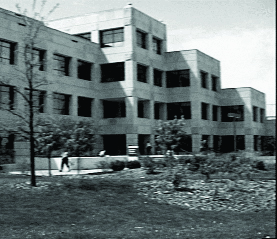
\includegraphics{Images/dc5}

% \isucaption{Durham Centre}
% \label{mgraph}
% \end{figure}

\subsubsection{Parts of the hypothesis}

Here one particular part of the hypothesis that is
currently being explained is examined and particular
elements of that part are given careful scrutiny.

% Below \subsubsection
% Sectional commands: \paragraph and \subparagraph may also be used

\subsection{Second Hypothesis}

Here one particular hypothesis is explained in depth
and is examined in the light of current literature.

\subsubsection{Parts of the second hypothesis}

Here one particular part of the hypothesis that is
currently being explained is examined and particular
elements of that part are given careful scrutiny.

\section{Criteria Review}

Here certain criteria are explained thus eventually
leading to a foregone conclusion.

%\chapterbib

%\bibliographystyle{apa}
%\bibliography{Reference/mybib}

% Chapter 5 from the standard thesis template
%   with a full page figure and a sideways table.
\chapter{SUMMARY AND DISCUSSION}

This is the opening paragraph to my thesis which
explains in general terms the concepts and hypothesis
which will be used in my thesis.

With more general information given here than really
necessary.

\section{Introduction}

Here initial concepts and conditions are explained and
several hypothesis are mentioned in brief.

Or graphically as seen in Figure~\ref{mgraph2}
it is certain that my hypothesis is true.

%\begin{figure}[p!] \centering

\begin{figure}[H] \centering % This goes with the package float comment this line out and use the previous one if you do not want to hold your position
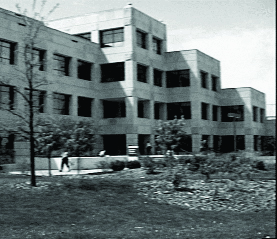
\includegraphics{Images/dc5}

\isucaption{Durham Centre---  Another View}
\label{mgraph2}
\end{figure}

\subsection{Hypothesis}

Here one particular hypothesis is explained in depth
and is examined in the light of current literature.

As can be seen in Table~\ref{nothingelse} it is
truly obvious what I am saying is true.

%\addtocontents{lot}{\protect\newpage}

\begin{sidewaystable} \centering
\isucaption{This table shows almost nothing but is a
sideways table and takes up a whole page by itself}
\label{nothingelse}
% Use: \begin{tabular{|lcc|} to put table in a box
\begin{tabular}{lcc} \hline
\textbf{Element} & \textbf{Control} & \textbf{Experimental} \\ \hline
Moon Rings & 1.23 & 3.38 \\
Moon Tides & 2.26 & 3.12 \\
Moon Walk & 3.33 & 9.29 \\ \hline
\end{tabular}
\end{sidewaystable}

\subsubsection{Parts of the hypothesis}

Here one particular part of the hypothesis that is 
currently being explained is examined and particular
elements of that part are given careful scrutiny.

% Below \subsubsection
% Sectional commands: \paragraph and \subparagraph may also be used

%\addtocontents{toc}{\protect\newpage} %% Remove this if needed, this lines forces the lines of the TOC starting with the below sub-heading "Critical Review" to go to the next page. Remove this formatting line as it will be required only if you want to force a table of contents entry to the next page along with the other subsequent entries.

\subsection{Second Hypothesis}

Here one particular hypothesis is explained in depth
and is examined in the light of current literature.

\subsubsection{Parts of the second hypothesis}

Here one particular part of the hypothesis that is 
currently being explained is examined and particular
elements of that part are given careful scrutiny.

\section{Criteria Review}

Here certain criteria are explained thus eventually
leading to a foregone conclusion.

\section{Results And Discussion}

Here the results can be inserted


%\chapterbib

%\bibliographystyle{apa}
%\bibliography{Reference/mybib}

%% Rearranging the table of contents to show references before appendix
%\unappendixtitle
%\addcontentsline{toc}{chapter}{REFERENCES} %this line is to be included before the last chapter so that in toc it appears after the last chapter. If you want the reference to be the last entry of the toc, remove this line and in the biblio.tex file insert this line (or uncomment the line  )

%% An example bibliography from the standard thesis template
\renewcommand{\bibname}{\centerline{REFERENCES}}
\unappendixtitle
\interlinepenalty=300
% For no page break use thebibnopage environment
\begin{thebibliography}{99}
%\begin{singlespacing}
\begingroup
    \setlength{\bibsep}{13.2pt}
  \linespread{1}\selectfont
\addcontentsline{toc}{chapter}{REFERENCESets}

\bibitem[Allen, B.~S.~(1984)]{allen}
Allen, B.~S. (1984). System-assigned learning strategies and CBI.
\emph{Journal of Instructional Computing Research},
\emph{1}(1), 3--18.
\filbreak

\bibitem[Bruner, J.~(1960)]{bruner}
Bruner, J. (1960). \emph{The process of education}.
New York: Random House.
\filbreak

\bibitem[Cox, S.~R.~(1974)]{cox}
Cox, S.~R. (1974). Computer-assisted instruction and student performance
in macroeconomic principles.
\emph{The Journal of Economic Education},
\emph{6}(1), 29--37.
\filbreak
%\end{singlespacing}
\end{thebibliography}

\renewcommand{\bibname}{\centerline{BIBLIOGRAPHY}}
\unappendixtitle
\interlinepenalty=300
\newpage
\phantomsection
\begingroup
    \setlength{\bibsep}{13.2pt}
  \linespread{1}\selectfont
\addcontentsline{toc}{chapter}{BIBLIOGRAPHY}
\bibliography{Reference/mybib}
\unappendixtitle
\endgroup



% Appendix1 file from standard thesis template

\appendixtitle 
\appendix


%% Use the following two lines for single appendix
%\unappendixtitle
%\singleappendixtitle

\chapter{ADDITIONAL MATERIAL} 
This is now the same as any other chapter except that
all sectioning levels below the chapter level must begin
with the *-form of a sectioning command.

\section*{More stuff}

Supplemental material.


% Instruction for single appendix check instruction in Appendix/appendix1.tex on top of the file
% An example second appendix from the example thesis thesis.tex.
\chapter{STATISTICAL RESULTS}

This is now the same as any other chapter except that
all sectioning levels below the chapter level must begin
with the *-form of a sectioning command.

\section*{Supplemental Statistics}

More stuff.


\end{document}

% IMPORTANT NOTES
% TABLE OF CONTENTS :
% TOPIC 1:  If you need a page break follow the steps below
% step1
% check before which chapter in the table of contents you want a page break
% step 2
% go the folder "body". There open the chapter tex file that you noted needed page break in the table of contents..
% step 3
% insert  \addtocontents{toc}{\protect\newpage} before the first line i.e. before the line \chapter{RESULTS}.

%%%%%%%%%%%%%%%%%%%%%%%%%%%%
% \def\@makechapterhead#1{%
% IN ORDER TO MAKE spacing changes in the title page got to the section in the isuthesis.cls file
% that starts with \long\def\maketitle{\begin{titlepage} and you can use options like
% singlespace (less spacing)
%singlespacing (comparitively more spacing almost like 2 spacing)
% onehalfspacing
%doublespacing (this is more spacing than the singlespacing above )
% more definitions on spacing can be found by going through the class file


% use \isucaption{} for all captions of figures and tables, where the captions are not too long.

% Use \isucaption[]{} with the square brackets for short caption of figure or table that goes into the list of tables and list of figures, and the curly brackets can have long captions which go with the figure/ table.

%%%%%% Using sub figures
% %%% In preamble include : \usepackage{subfig}
% \begin{figure}[htbp]
% 	\centering
% 	\subfloat[first caption.\label{fig:2a}]{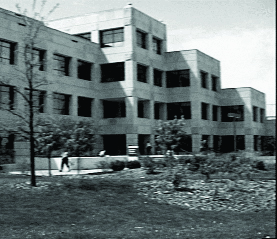
\includegraphics[width=0.2\textwidth]{Images/dc5.jpg}}\hfill
%     \subfloat[second caption.\label{fig:2b}] {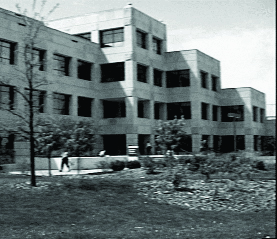
\includegraphics[width=0.2\textwidth]{Images/dc5.jpg}}\hfill
% 	\isucaption{Sub-figure test}
% 	\label{fig:subfigure-test}
% \end{figure}

% Subfloat reference: Fig \ref{fig:2a}

% Figure reference: Fig \ref{fig:subfigure-test}
